\chapter{Arhitektura i dizajn sustava}
		
		\textbf{\textit{dio 1. revizije}}\\

		\textit{ Potrebno je opisati stil arhitekture te identificirati: podsustave, preslikavanje na radnu platformu, spremišta podataka, mrežne protokole, globalni upravljački tok i sklopovsko-programske zahtjeve. Po točkama razraditi i popratiti odgovarajućim skicama:}
	\begin{itemize}
		\item 	\textit{izbor arhitekture temeljem principa oblikovanja pokazanih na predavanjima (objasniti zašto ste baš odabrali takvu arhitekturu)}
		\item 	\textit{organizaciju sustava s najviše razine apstrakcije (npr. klijent-poslužitelj, baza podataka, datotečni sustav, grafičko sučelje)}
		\item 	\textit{organizaciju aplikacije (npr. slojevi frontend i backend, MVC arhitektura) }		
	\end{itemize}
	
		\section{Baza podataka}
			
			Kao sustav upravljanja bazom podataka koristimo PostgreSQL \textit{Sustav za Upravljanje Bazom Podataka} (SUBP). Na bazu se spajamo putem \textit{Java DataBase Connectivity} (JDBC) specifikacije, koja omogućuje Java programima spajanje na SUBP i njegovo korištenje. Na JDBC specifikaciju nadograđuje se \textit{Java Persistence API} (JPA) koji pruža usluge \textit{Object-Relational Mapping} (ORM), čime se odabrani Java objekti automatski spremaju u bazu podataka.
		
			\subsection{Opis tablica}
			
				U bazi podataka nalazi se 9 relacija:
				\begin{packed_item}
					\item \textbf{Persons} - relacija koja opisuje osobu u najširem smislu; osoba može biti korisnik aplikacije, komunalni radnik ili administrator sustava, te se u ovoj relaciji spremaju zajednički atributi tih aktora
					\item \textbf{Admins} - relacija u kojoj se nalaze zapisi svih administratora
					\item \textbf{Employees} - relacija u kojoj se nalaze zapisi svih komunalnih radnika
					\item \textbf{Citizens} - relacija u kojoj se nalaze zapisi svih građana - regularnih korisnika aplikacije
					\item \textbf{Container} - relacija u kojoj su spremljeni zapisi o kontejnerima
					\item \textbf{Neighborhoods} - relacija u kojoj su spremljeni zapisi o susjedstvima
					\item \textbf{Favorites} - relacija u kojoj su spremljeni zapisi o parovima Person-Container, sa značenjem da je osoba Person spremila kontejner Container radi brzog pristupa.
					\item \textbf{Pings} - relacija u kojoj su spremljeni zapisi o parovima Person-Container, sa značenjem da je osoba Person prijavila kontejner Container kao pun, pretrpan ili prazan.
					\item \textbf{Emptyings} - relacija u kojoj su spremljeni zapisi o pražnjenjima kontejnera oblika Employee-Container, sa značenjem da je radnik Employee ispraznio kontejner Container
				\end{packed_item}
			
				Tablica Person je generička tablica za osobu, a nju nasljeđuju tablice Admin, Employee i Citizen, svaki sa svojim dodatnim atributima te stranim ključem koji pokazuje na tablicu Person gdje se nalaze zajednički atributi svojstveni svima trima entitetima.	Tablice Favorites, Pings i Emptyings su tablice koje postoje kako bi se opisala N-N veza između relacija koje povezuju.


			\subsection{Definicije tablica}
				\begin{longtabu} to \textwidth {|X[6, l]|X[6, l]|X[20, l]|}
					
					\hline \multicolumn{3}{|c|}{\textbf{Person}}	 \\[3pt] \hline
					\endfirsthead
					
					\hline \multicolumn{3}{|c|}{\textbf{Person}}	 \\[3pt] \hline
					\endhead
					
					\hline 
					\endlastfoot
					
					\cellcolor{LightGreen}id & BIGINT	&   Identifikator osobe; svaka osoba ima svoj jedinstveni ID	\\ \hline
					name	& VARCHAR &   Ime osobe, ne smije biti NULL	\\ \hline 
					last\textunderscore name & VARCHAR & Prezime osobe, ne smije biti NULL \\ \hline
					email & VARCHAR &  E-mail osobe, koristi se pri prijavi korisnika u sustav, ne smije biti NULL i jedinstvena je vrijednost \\ \hline 
					pwd\textunderscore hash & VARCHAR	&  \textit{Digest} lozinke koju je osoba odabrala \\ 
					
				\end{longtabu}
			
				\begin{longtabu} to \textwidth {|X[6, l]|X[6, l]|X[20, l]|}
					
					\hline \multicolumn{3}{|c|}{\textbf{Admin}}	 \\[3pt] \hline
					\endfirsthead
					
					\hline \multicolumn{3}{|c|}{\textbf{Admin}}	 \\[3pt] \hline
					\endhead
					
					\hline 
					\endlastfoot
					
					\cellcolor{LightBlue}id & BIGINT	&   Jedini atribut tablice - strani ključ koji pokazuje na tablicu Person.	\\ 
					
				\end{longtabu}
			
				\begin{longtabu} to \textwidth {|X[6, l]|X[6, l]|X[20, l]|}
					
					\hline \multicolumn{3}{|c|}{\textbf{Citizen}}	 \\[3pt] \hline
					\endfirsthead
					
					\hline \multicolumn{3}{|c|}{\textbf{Citizen}}	 \\[3pt] \hline
					\endhead
					
					\hline 
					\endlastfoot
					
					\cellcolor{LightBlue}id & BIGINT	&   Strani ključ koji pokazuje na tablicu Person.	\\ \hline
					reputation & INT & Atribut koji označava reputaciju korisnika; služi za procjenu vjerodostojnosti njegove prijave. \\
					
				\end{longtabu}
			
				\begin{longtabu} to \textwidth {|X[7, l]|X[7, l]|X[20, l]|}
					
					\hline \multicolumn{3}{|c|}{\textbf{Employee}}	 \\[3pt] \hline
					\endfirsthead
					
					\hline \multicolumn{3}{|c|}{\textbf{Employee}}	 \\[3pt] \hline
					\endhead
					
					\hline 
					\endlastfoot
					
					\cellcolor{LightBlue}id & BIGINT	&   Strani ključ koji pokazuje na tablicu Person.	\\ \hline
					oib & VARCHAR(11) & OIB komunalnog radnika. \\ \hline
					\cellcolor{LightBlue} neighborhood\textunderscore id & BIGINT & Strani ključ koji pokazuje na tablicu Neighborhood. Određuje kojem kvartu pripada radnik. \\
					
				\end{longtabu}
			
				\begin{longtabu} to \textwidth {|X[7, l]|X[7, l]|X[20, l]|}
					
					\hline \multicolumn{3}{|c|}{\textbf{Container}}	 \\[3pt] \hline
					\endfirsthead
					
					\hline \multicolumn{3}{|c|}{\textbf{Container}}	 \\[3pt] \hline
					\endhead
					
					\hline 
					\endlastfoot
					
					\cellcolor{LightGreen}id & BIGINT	&   Identifikator kontejnera; svaki kontejner ima svoj jedinstveni ID	\\ \hline
					latitude & DOUBLE & Geografska širina lokacije kontejnera \\ \hline
					longitude & DOUBLE & Geografska dužina lokacije kontejnera \\ \hline
					pings\textunderscore since\textunderscore emptied & INT & Broj prijava kontejnera od njegovog zadnjeg pražnjenja \\ \hline
					\cellcolor{LightBlue} neighborhood\textunderscore id & BIGINT & Strani ključ koji pokazuje na tablicu Neighborhood. Određuje u kojem se kvartu nalazi kontejner. \\
					
				\end{longtabu}
		
			\begin{longtabu} to \textwidth {|X[7, l]|X[7, l]|X[20, l]|}
				
				\hline \multicolumn{3}{|c|}{\textbf{Neighborhood}}	 \\[3pt] \hline
				\endfirsthead
				
				\hline \multicolumn{3}{|c|}{\textbf{Neighborhood}}	 \\[3pt] \hline
				\endhead
				
				\hline 
				\endlastfoot
				
				\cellcolor{LightGreen}id & BIGINT	&   Identifikator susjedstva; svako susjedstvo (kvart) ima svoj jedinstveni ID	\\ \hline
				latitude & DOUBLE & Geografska širina lokacije komunalnog središta u susjedstvu \\ \hline
				longitude & DOUBLE & Geografska dužina lokacije komunalnog središta u susjedstvu \\ \hline
				name & VARCHAR & Ime susjedstva \\
				
			\end{longtabu}
		
			\begin{longtabu} to \textwidth {|X[7, l]|X[7, l]|X[20, l]|}
				
				\hline \multicolumn{3}{|c|}{\textbf{Favorites}}	 \\[3pt] \hline
				\endfirsthead
				
				\hline \multicolumn{3}{|c|}{\textbf{Favorites}}	 \\[3pt] \hline
				\endhead
				
				\hline 
				\endlastfoot
				
				\cellcolor{LightGreen}id & BIGINT	&   Identifikator oznake favorita; svako označavanje ima svoj jedinstveni ID. \\ \hline
				\cellcolor{LightBlue} container\textunderscore id & BIGINT & Strani ključ koji pokazuje na relaciju Container \\ \hline
				\cellcolor{LightBlue} owner\textunderscore id & BIGINT & Strani ključ koji pokazuje na relaciju Person  \\
				
			\end{longtabu}
		
			\begin{longtabu} to \textwidth {|X[7, l]|X[7, l]|X[20, l]|}
				
				\hline \multicolumn{3}{|c|}{\textbf{Pings}}	 \\[3pt] \hline
				\endfirsthead
				
				\hline \multicolumn{3}{|c|}{\textbf{Pings}}	 \\[3pt] \hline
				\endhead
				
				\hline 
				\endlastfoot
				
				\cellcolor{LightGreen}id & BIGINT	&   Identifikator prijave; svako označavanje ima svoj jedinstveni ID. \\ \hline
				level & INT & Level koji označava vrstu prijave: 0 je prijava praznog, 1 prijava punog i 2 prijava pretrpanog kontejnera \\ \hline
				timestamp & BIGINT & Vremenska oznaka trenutka u kojem se dogodila prijava kontejnera \\ \hline
				photo\textunderscore path & VARCHAR & Mjesto na disku na kojem se nalazi fotografija koju je priložio korisnik \\ \hline
				\cellcolor{LightBlue} container\textunderscore id & BIGINT & Strani ključ koji pokazuje na relaciju Container \\ \hline
				\cellcolor{LightBlue} owner\textunderscore id & BIGINT & Strani ključ koji pokazuje na relaciju Person  \\
				
			\end{longtabu}
		
			\begin{longtabu} to \textwidth {|X[7, l]|X[7, l]|X[20, l]|}
				
				\hline \multicolumn{3}{|c|}{\textbf{Pings}}	 \\[3pt] \hline
				\endfirsthead
				
				\hline \multicolumn{3}{|c|}{\textbf{Pings}}	 \\[3pt] \hline
				\endhead
				
				\hline 
				\endlastfoot
				
				\cellcolor{LightGreen}id & BIGINT	&   Identifikator prijave; svako označavanje ima svoj jedinstveni ID. \\ \hline
				level & INT & Level koji označava vrstu prijave: 0 je prijava praznog, 1 prijava punog i 2 prijava pretrpanog kontejnera \\ \hline
				timestamp & BIGINT & Vremenska oznaka trenutka u kojem se dogodila prijava kontejnera \\ \hline
				photo\textunderscore path & VARCHAR & Mjesto na disku na kojem se nalazi fotografija koju je priložio korisnik \\ \hline
				\cellcolor{LightBlue} container\textunderscore id & BIGINT & Strani ključ koji pokazuje na relaciju Container \\ \hline
				\cellcolor{LightBlue} creator\textunderscore id & BIGINT & Strani ključ koji pokazuje na relaciju Person  \\
				
			\end{longtabu}
		
			\begin{longtabu} to \textwidth {|X[7, l]|X[7, l]|X[20, l]|}
				
				\hline \multicolumn{3}{|c|}{\textbf{Emptyings}}	 \\[3pt] \hline
				\endfirsthead
				
				\hline \multicolumn{3}{|c|}{\textbf{Emptyings}}	 \\[3pt] \hline
				\endhead
				
				\hline 
				\endlastfoot
				
				\cellcolor{LightGreen}id & BIGINT	&   Identifikator prijave; svako označavanje ima svoj jedinstveni ID. \\ \hline
				timestamp & BIGINT & Vremenska oznaka trenutka u kojem se dogodila prijava kontejnera \\ \hline
				\cellcolor{LightBlue} container\textunderscore id & BIGINT & Strani ključ koji pokazuje na relaciju Container \\ \hline
				\cellcolor{LightBlue} worker\textunderscore id & BIGINT & Strani ključ koji pokazuje na relaciju Employee  \\
				
			\end{longtabu}
			
			
			\subsection{Dijagram baze podataka}
				\begin{figure}[H]
					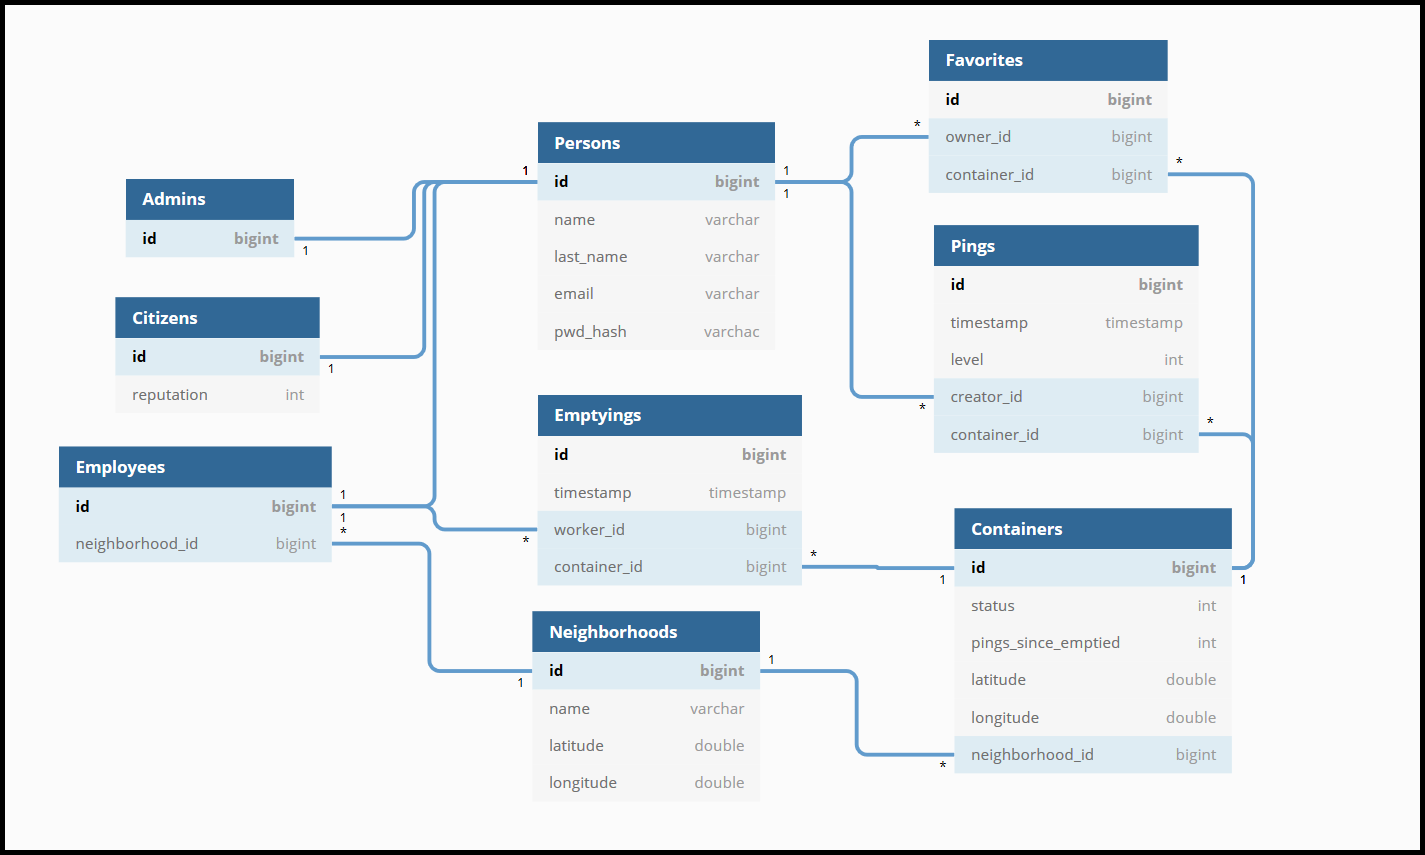
\includegraphics[scale=0.5]{figures/db_diagram.PNG}
					\centering
					\caption{Dijagram baze podataka}
					\label{fig:db-diag}
				\end{figure}
			
				\begin{figure}[H]
					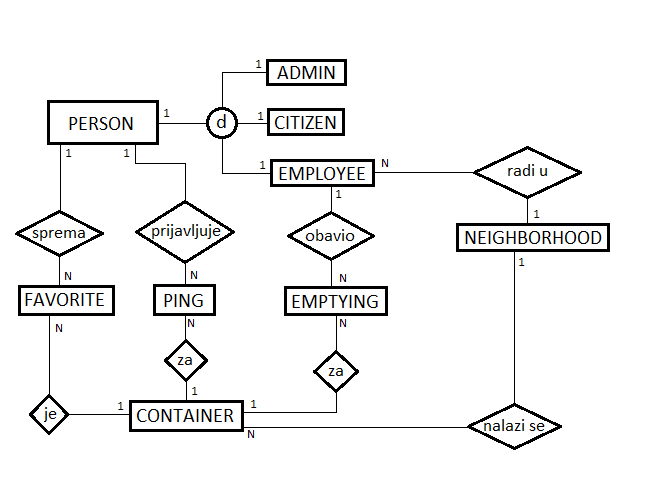
\includegraphics[scale=0.8]{figures/er_model.PNG}
					\centering
					\caption{Entitetsko-Relacijski model baze podataka}
					\label{fig:er-model}
				\end{figure}
			
			\eject
			
			
		\section{Dijagram razreda}
		
			\textit{Potrebno je priložiti dijagram razreda s pripadajućim opisom. Zbog preglednosti je moguće dijagram razlomiti na više njih, ali moraju biti grupirani prema sličnim razinama apstrakcije i srodnim funkcionalnostima.}\\
			
			\textbf{\textit{dio 1. revizije}}\\
			
			\textit{Prilikom prve predaje projekta, potrebno je priložiti potpuno razrađen dijagram razreda vezan uz \textbf{generičku funkcionalnost} sustava. Ostale funkcionalnosti trebaju biti idejno razrađene u dijagramu sa sljedećim komponentama: nazivi razreda, nazivi metoda i vrste pristupa metodama (npr. javni, zaštićeni), nazivi atributa razreda, veze i odnosi između razreda.}\\
			
			\textbf{\textit{dio 2. revizije}}\\			
			
			\textit{Prilikom druge predaje projekta dijagram razreda i opisi moraju odgovarati stvarnom stanju implementacije}
			
			
			
			\eject
		
		\section{Dijagram stanja}
			
			
			\textbf{\textit{dio 2. revizije}}\\
			
			\textit{Potrebno je priložiti dijagram stanja i opisati ga. Dovoljan je jedan dijagram stanja koji prikazuje \textbf{značajan dio funkcionalnosti} sustava. Na primjer, stanja korisničkog sučelja i tijek korištenja neke ključne funkcionalnosti jesu značajan dio sustava, a registracija i prijava nisu. }
			
			
			\eject 
		
		\section{Dijagram aktivnosti}
			
			\textbf{\textit{dio 2. revizije}}\\
			
			 \textit{Potrebno je priložiti dijagram aktivnosti s pripadajućim opisom. Dijagram aktivnosti treba prikazivati značajan dio sustava.}
			
			\eject
		\section{Dijagram komponenti}
		
			\textbf{\textit{dio 2. revizije}}\\
		
			 \textit{Potrebno je priložiti dijagram komponenti s pripadajućim opisom. Dijagram komponenti treba prikazivati strukturu cijele aplikacije.}